\subsection{Definitions}
\begin{definition}[Signal Energy]
\[E_x = \int_{-\infty}^{\infty} |x(t)|^2dt \]
\end{definition}

\begin{definition} [Siganl Power]
    \[P_x = lim_{T \to \infty} \frac{1}{T} \int_{-T/2}^{T/2} |x(t)|^2dt\]
\end{definition}

\begin{definition} [Time Shifting]
    \[\phi(t + T) = x(t)\]
    \[\phi(t) = x(t - T)\]
    $x(t-T)$ represents $x(t)$ time shifted by T seconds.  
\end{definition}

\section{Classification of Signals}
I felt like 330 never really laid out the these basic ideas about siganls in a good way. For example, I remember Micheal and I didn't realize that anytime a signal is said to be from convolution, it is a LTI system.
\begin{figure}[h]
    \centering
    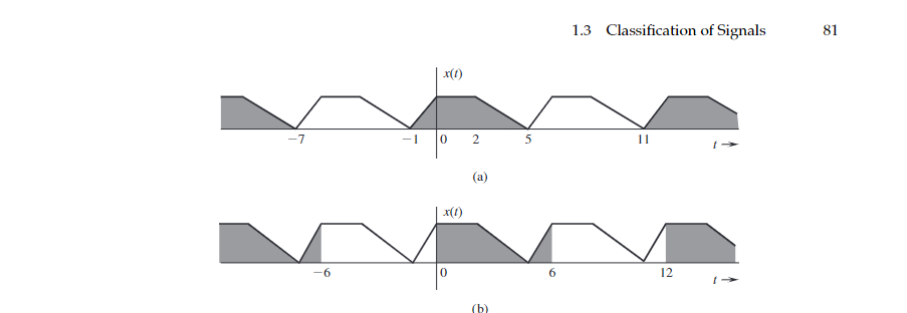
\includegraphics[width = 0.75\textwidth]{images/properties_example_1.3.png}
    \caption{Example of a property}
    \label{fig:properties_example}
\end{figure}

I like how the book goes over basic signal properites like time shifts, reversals, etc. instead of properites being introduced randomly throughout the semester (this is done well with fourier).

\begin{figure}
    \center 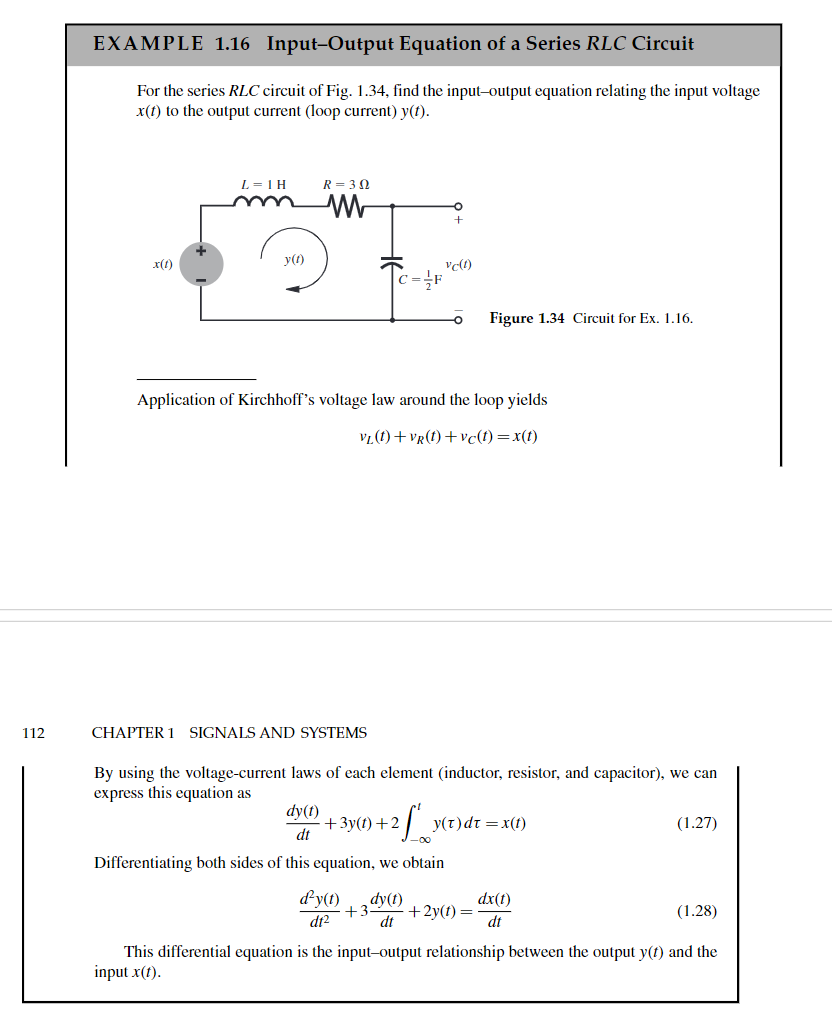
\includegraphics[width = 0.5\textwidth]{images/circuit_input_output_example.png}
\end{figure}

\begin{example} [\textbf{Unit Step Matlab Code}]
    I think students are intially confused by the idea of using the unit step function to represent other signals such as a rectangle. Might be nice to have a little matlab script.

    \begin{center}
        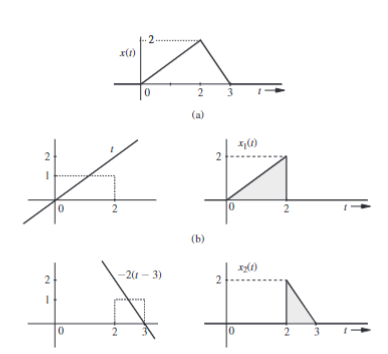
\includegraphics{images/function_w_unitstep_1.7.png}
    \end{center}
    \[x_1(t) = t[u(t) - u(t-2)]\]
    \[x_2(t) = -2(t-3)[u(t-2)-u(t-3)]\]
    \[x(t) = x_1(t) + x_2(t)\]

    Example 1.7 and drill 1.7, 1.8 are all good examples of using unit step.
\end{example}

\subsection{The Exponential Function}
\textbf{We could wait to explain this when we do Laplace.}
\subsection{Even and Odd Functions}
\textbf{Useful but seems out of place/not needed considering how much content there is to cover.}

\section{Systems}
\begin{example}
    \begin{center}
        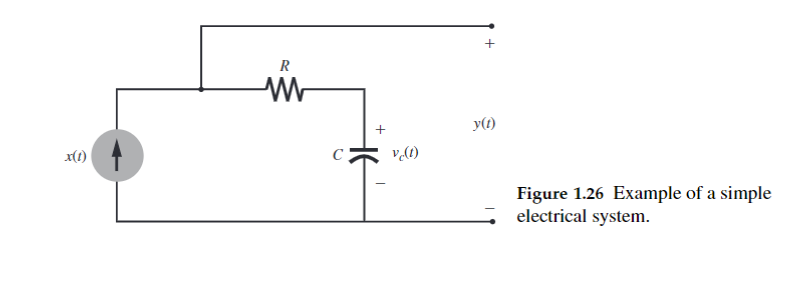
\includegraphics{images/circuits_as_system.png}
    \end{center}
    I think we should try to add a lot more circuit examples. Most students should have taken 230 by then or Physics 2.
\end{example}

\section{Classification of Systems}
Again, I think its a good idea to clearer go over all these system properties in a clear manner.

\begin{center}
    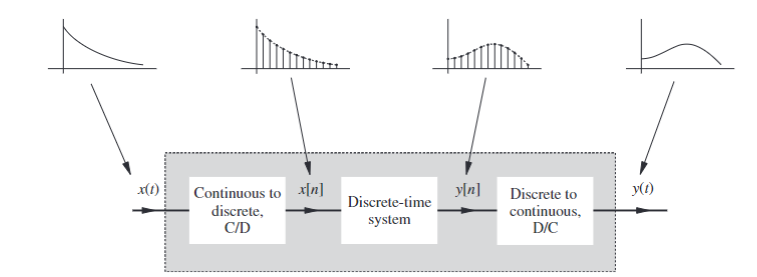
\includegraphics{images/difference_of_discrete_cont.png}
\end{center}
This is a good figure.

The end of the chapter has a lot of circuit examples that seem good.
